\section{Durchführung}
\label{sec:Durchführung}
\subsection{Aufbau}
Der Aufbau der Messapparatur wird in Abbildung \ref{fig:auf} dargestellt. Ein Geiger-Müller Zählrohr detektiert dabei die emittierten $\beta$- und $\gamma$-Teilchen.
Das Zählrohr befindet sich mit der Probe in einer Bleiabschirmung, so dass der Nulleffekt möglichst gering ausfällt. Jedes detektierte Teilchen liefert am Verstärkerausgang einen elektrischen Impuls, welcher an das Zählwerk weitergeleitet wird.  
\begin{figure}
    \centering
    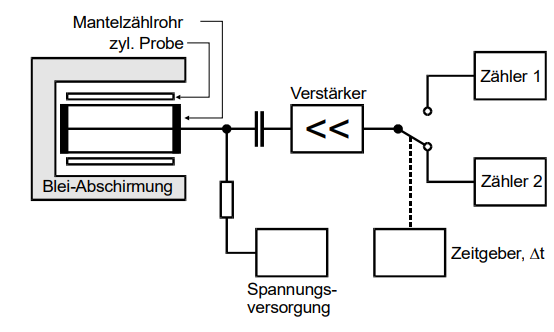
\includegraphics[scale=0.6]{content/Aufbau.png}
    \caption{Schematische Darstellung des Versuchsaufbaus \cite{v703}}
    \label{fig:auf}
  \end{figure}
  \subsection{Messung}
  Zuerst wird die Untergrundrate $N_\text{U}$ siebenfach gemessen, wobei das Messintervall $t=\SI{300}{\second}$ gewählt wurde. 
  Der Versuch wurde mit Vanadium und Rhodium durchgeführt. Die Proben werden direkt nach Entnehmen aus der Neutronenquelle auf das Geiger-Müller Zählrohr gesteckt.
  Die Messung des Vanadiums wurde mit einem Messintervall von $\symup{\Delta}t=\SI{30}{\second}$ durchgefüht;
  die des Rhodiums mit einem Intervall von $\symup{\Delta}t=\SI{15}{\second}$. Nach $\SI{1230}{\second}$ wird die Messung mit dem Vanadium beendet.
  Die Messung mit der Rhodiumprobe wurde nach $\SI{630}{\second}$ beendet.